\section{Ideal Spectra from Single-Chirp Excitation}
\label{sec:bbqchili}
There are numerous nuclei of interest in \ac{NMR} with very wide chemical shift
ranges, including \ch{^{19}F} (of particular interest in the pharmaceutical
industry), \ch{^{31}P}, and \ch{^{195}Pt}.
Attaining spectra covering the entire chemical shift range of such nuclei for
use in quantitative applications is challenging due to off-resonance effects,
which severely alter the amplitudes and phases of resonances with frequencies
far from that of the transmitter~\cite[Section 3.4.1]{Cavanagh2007}. One
popular means of achieving ultra-broadband excitation, in which a consistent
amplitude- and phase-profile across a spectral window of tens or even hundreds
of \unit{\kilo\hertz} the achieved, is to use \ac{FS} pulses, during
which the frequency of \ac{RF} irradiation varies with
time~\cite{Foroozandeh2020}. One of the most common classes of \ac{FS} pulses
are those where the variation of excitation frequency with time is linear, with
such pulses commonly referred to as \emph{chirp} pulses. The application of a
single \ang{90} chirp pulse to achieve ultra-broadband excitation, while
involving a simple and short pulse sequence, yields
spectra with undesirable phase behaviour, on account of resonances with
different frequencies being excited at different moments in time.
There are well-established methods for overcoming this using
pulse sequences featuring an initial excitation, followed by one or more
refocussing \ac{FS}
pulses~\cite{Bohlen1989,Bohlen1993,Cano2002,Power2016,Foroozandeh2019}.

With knowledge of the form of the chirp pulse, the expected phase of a
particular signal is determinable, and in this section, it will be shown
that well-phased spectra can be obtained from excitation with a single \ac{FS}
pulse when appropriate post-processing of the \ac{FID} is employed.
The main advantage of being able to derive spectra with desirable features from
a single chirp excitation experiment is the fact that ultra-broadband spectra
can be generated using a far shorter pulse sequence than state of the art
methods such as \ac{CHORUS}~\cite{Power2016,Foroozandeh2019}, where both a
\ang{90} chirp pulse, and two \ang{180} chirp pulses are applied; spectra with
improved signal intensity could therefore be realised. Here, a description of the
technique is presented, followed by an illustration of its performance on both a
simulated and an experimental dataset.

\subsection{Chirp Excitation}
\begin{figure}
    \centering
    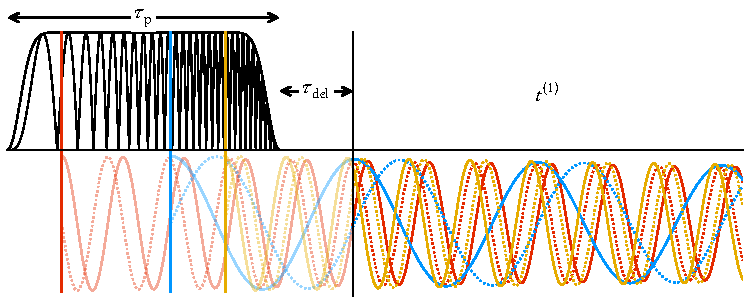
\includegraphics{single_chirp_illustration/single_chirp_illustration.pdf}
    \caption[
        An illustration of an experiment comprising a single chirp pulse.
    ]
    {
        An illustration of an experiment comprising a single chirp pulse sweeping
        low to high frequencies of duration $\tau_{\text{p}}$, followed by
        a pre-scan delay period of time $\tau_{\text{del}}$, prior to
        acquisition. The fate of three resonances with different frequencies is
        denoted, with $f_{\text{red}} < f_{\text{blue}} <
        f_{\text{yellow}}$. Each resonance is excited at different points
        in time, with lower frequency resonances being excited earlier, such that
        each of these evolves for different amounts of time prior
        to acquisition ($\tau_0$).
        The resulting \ac{FID} comprises signals whose phases depend on their
        frequencies quadratically.
        Coloured oscillations denote the evolution of each resonance, with
        solid and dashed lines representing real and imaginary components,
        respectively. It is assumed that the pulse rotates each
        resonance so as to be in phase with the receiver at the point of
        excitation.
    }
    \label{fig:single-chirp}
\end{figure}
Focus is limited here to chirp pulses which sweep from low to high
frequencies; they are parameterised by
their duration $\tau_{\text{p}}$ (\unit{\second}),
excitation bandwidth $\Updelta F$ (\unit{\hertz}),
and \ac{RF} ``amplitude'' $\omega_{\text{RF}}$ (\unit{\hertz}).
The frequencies that a pulse sweeps through are in the range
$[\foff - \nicefrac{1}{2} \Updelta F,
\foff + \nicefrac{1}{2} \Updelta F]$,
and the rate at which the frequency of the chirp is increased (the sweep
rate) is given by $\nicefrac{\Updelta F}{\tau_{\text{p}}}$.
\Cref{fig:single-chirp} provides an illustration of a single chirp
excitation experiment. After application of the chirp pulse, there is typically
a short pre-scan delay $\tau_{\text{del}}$, usually on the order of a few
\unit{\micro\second}, prior to the start of acquisition. While the pre-scan
delay can be determined if an intimate knowledge of the spectrometer hardware
is known, this varies from instrument to instrument, and is not trivial to
ascertain. It is this delay which induces a first-order phase shift in \ac{NMR}
experiments, and which is routinely corrected for by phase correction.
The various chirp pulse parameters are inter-related as
follows~\cite{Foroozandeh2019,Kupce1995b}:
\begin{equation}
    \omega_{\text{RF}} = \sqrt{
        \frac{\Updelta F Q}{2 \pi \tau_{\text{p}}}
    },
\end{equation}
where $Q \in \mathbb{R}_{>0}$ is the \emph{adiabaticity factor}.
For a pulse with flip angle  $\beta < \ang{180}$, $Q$ is related to $\beta$ via
\begin{equation}
    Q = \frac{2}{\pi} \ln \left( \frac{2}{\cos(\beta) + 1} \right),
\end{equation}
such that an appropriate pulse to achieve a flip angle of \ang{90} requires
selecting a combination of $\omega_{\text{RF}}$, $\Updelta F$, and
$\tau_{\text{p}}$ which satisfies $Q \approx 0.441$.
The combination used in examples in this work is $\Updelta F =
\qty{400}{\kilo\hertz}$, $\tau_{\text{p}} = \qty{100}{\micro\second}$, and
$\omega_{\text{RF}} \approx \qty{16.8}{\kilo\hertz}$.
For a pulse with sufficiently low $\omega_{\text{RF}}$\,---\,this requires a
sufficiently large pulse duration for a given excitation bandwidth\,---\,it is
reasonable to assume that the chirp pulse induces an instantaneous \ang{90}
rotation at the point of resonance, as depicted in
\cref{fig:single-chirp}. As such, resonances with different
Larmor frequencies evolve for different amounts of time prior to the start of
acquisition, according to
\begin{equation}
    \tau_0\left(f\right) =
        \tau_{\text{del}} + \frac{\tau_{\text{p}}}{2} -
        \frac{(f - \foff) \tau_{\text{p}}}{2 \Updelta F}.
    \label{eq:t0}
\end{equation}
$\tau_{\text{del}} + \nicefrac{\tau_{\text{p}}}{2}$ is the amount of time
between excitation and detection for the on-resonance case, in which
excitation occurs exactly halfway through the pulse. Resonances
with a frequency smaller than that of the transmitter are excited earlier and hence
have a larger $\tau_0$, while the converse is true for resonances with greater
frequencies. The resulting overall phase as of a signal a function of its
frequency can be approximated as~\cite{Foroozandeh2019}
\begin{equation}
    \phi(f) = \phi_0 + 2 \pi \left(\tau_{\text{del}} + \frac{\tau_{\text{p}}}{2} \right) (f - \foff) -
        2 \pi \left(\frac{\tau_{\text{p}}}{2 \Updelta F}\right)
        (f - \foff)^2.
    \label{eq:quadratic-phase}
\end{equation}
One might assume that it is possible to generate phased spectra by simply
applying phase correction to the spectrum generated, via
\begin{equation}
    s_{\phi}(f) = s(f) \exp(-\iu \phi(f)).
        \label{eq:spec-phase-chili}
\end{equation}
While the quadratic phase behaviour of peaks is corrected by doing this,
another issue with the dataset is not addressed;
for any resonance, the signal that is detected can be thought of as
the difference between two signals:
\begin{enumerate}
    \item The ``complete'' signal, which starts at the time of excitation.
    \item A ``truncated'' signal which is identical to the complete signal
        before acquisition, and which comprises zeros once acquisition has
        begun.
\end{enumerate}
The linear nature of the \ac{FT} dictates that the
resulting delayed-acquisition spectrum comprises the difference between the
\acp{FT} of the complete signal and the truncated signal.  The \ac{FT} of a
severely
truncated \ac{FID} comprises a broad sinc function with its maximum
at the signal frequency. The appearance of the sinc wiggle depends on
the gap between excitation and acquisition; resonances of lower
frequencies will exhibit deeper, narrower artefacts since the signal is more
significantly truncated. The result of applying quadratic phase correction is
therefore a spectrum of well-phased peaks, but with major baseline distortions,
particularly in the low-frequency region. Figures \ref{fig:bbqchili-sim}.b and
\ref{fig:bbqchili-real}.b both provide examples of this phenomenon.

\subsection{Methodology}
Both the quadratic phase behaviour and delay-induced baseline distortions can
be resolved if an estimate of the \ac{FID}'s parameters is obtained. This enables
the construction of a synthetic \ac{FID} featuring oscillators which are
back-propagated, such that they begin not at the point of acquisition, but at
the point of excitation. The appropriate start time for an oscillator with
frequency $f$ is given by $-\tau_0$, with $\tau_0$ defined in \cref{eq:t0}. The
resulting corrected \ac{FID} $\by \in \mathbb{C}^N$ is defined as
\begin{equation}
    y_n = \sum_{m=1}^{M} \amexpphim \exp((2 \pi \iu (f_m - \foff) - \eta_m) (n \Dt - \tau_0(f_m)))\quad
        \forall n \in \lbrace 0, \cdots, N-1 \rbrace.
    \label{eq:backprop}
\end{equation}
This concept has similarities to the use of \ac{LP} in order to back-propagate
an \ac{FID} to correct for corrupted initial points. However, a holistic
approach such as \ac{LP} cannot be used in this application, as each signal
component must be treated differently according to its frequency.

Thus far in this work, it has been assumed that all signals which make up a
dataset are of the same phase. Of course this isn't the case for \acp{FID}
generated from single-chirp excitation. As such, it is inappropriate to
incorporate the variance of oscillator phases in the fidelity for \ac{NLP}.
For the examples presented in this section, \ac{NLP} was not applied at all;
the direct output of the \ac{MPM} was used as the estimate of the \acp{FID}
parameters.

\subsection{Results}
\begin{figure}
    \centering
    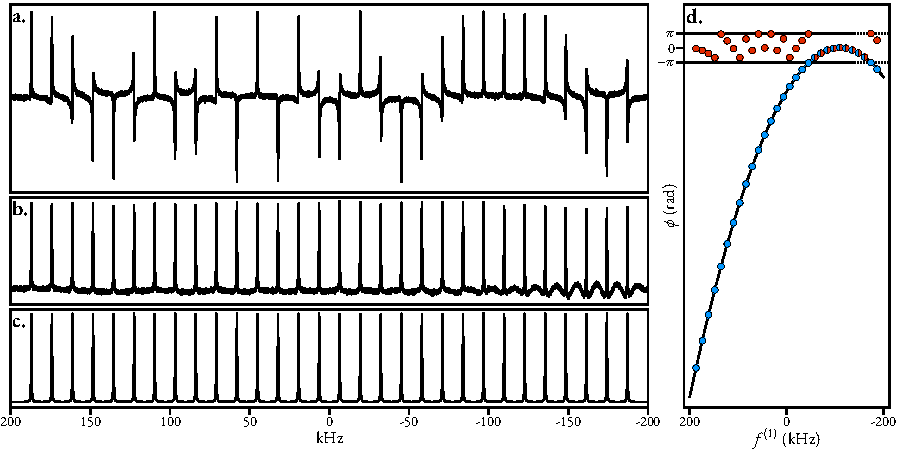
\includegraphics{chirp_phase_vs_estimation/chirp_phase_vs_estimation.pdf}
    \caption[
        A comparison of quadratic phase correction vs frequency-dependent
        back-propagation in treating simulated single-chirp excitation data.
    ]
    {
        A comparison of quadratic phase correction vs frequency-dependent
        back-propagation in treating simulated single-chirp excitation data.
        \textbf{a.} Simulated spectrum for a spin system comprising 30 spins
        with uniformly-separated resonance frequencies. The data were generated
        with
        $N=2^{14}$,
        $\fsw=\qty{400}{\kilo\hertz}$,
        $\foff=\qty{0}{\hertz}$,
        $\tau_{\text{p}} = \qty{100}{\micro\second}$,
        $\tau_{\text{del}} = \qty{0}{\second}$,
        $\Updelta F = \qty{400}{\kilo\hertz}$.
        Coloured lines depict individual oscillators generated using the
        \ac{MPM}; these have been slightly offset for clarity.
        \textbf{b.} Spectrum generated using quadratic phase correction
        (\cref{eq:spec-phase-chili}).
        \textbf{c.} Spectrum generated using the back-propagation approach.
        \textbf{d.} Estimated phases of each oscillator as a function of
        frequency. Red points: phases wrapped within the range $(-\pi, \pi]$.
        Blue points: the same phases, adjusted by addition of a suitable multiple
        of $2 \pi$ to each red point in order to display their quadratic
        dependence on frequency.
        Black curve: quadratic fit of the blue points. The equation of the
        quadratic is stated.
    }
    \label{fig:bbqchili-sim}
\end{figure}
\Cref{fig:bbqchili-sim,fig:bbqchili-real} present comparisons
between the application of quadratic phase correction and the proposed
back-propagation procedure. In the former, a simulated
dataset is considered, comprising 30 evenly-spaced signals, and generated using
\cref{eq:backprop} with $-\tau_0(f_m)$ replaced with $+\tau_0(f_m)$. Other
relevant parameters used are stated in the caption.
A very large damping factor ($\qty{1000}{\per\second}$) was assigned to each
oscillator, as this augments the baseline distortions in the spectrum.
\ac{AWGN} was added to the \ac{FID}, with a target \ac{SNR} of
\qty{25}{\deci\bel}.

The spectrum after quadratic phase correction (\cref{fig:bbqchili-sim}.b)
exhibits the undesired baseline distortions as discussed, with more intense,
narrower baseline distortions associated with lower-frequency signals.
The \ac{MPM} was used to estimate the \ac{FID}'s parameters,
with only the first 2048 points considered
Performing the \ac{MPM} on a signal with $2^{14}$ points would take (a) a
long time, and (b) require a very large amount of \ac{RAM} (see Figures
\ref{fig:mpm-profiling}.a1 and \ref{fig:mpm-profiling}.a2).
Estimating a truncated \ac{FID} comprising the first 2048 points of the
data is justifiable here, since all signal frequencies are spaced
reasonably far apart, meaning each signal in the \ac{FID} becomes
resolvable from the others early on into evolution.
The spectrum generated via back-propagation is presented in
\cref{fig:bbqchili-sim}.c, which is well-phased, and does not suffer from
baseline distortion. The variation of the estimated oscillator
phases against their frequencies is plotted in \cref{fig:bbqchili-sim}.d, with
the quadratic dependence clearly illustrated; fitting the blue points to a
quadratic function yielded a second-order coefficient of
$\qty{-7.85e-10}{\radian\second\squared}$, in agreement with the expected value
of $-2 \pi \left(\nicefrac{\tau_{\text{p}}}{2 \Updelta F}\right)$.

\Cref{fig:bbqchili-real} features an experimental dataset, acquired
from a sample of 1\% \ch{Gd}-doped \ch{H2O} in \ch{D2O}\footnote{
    The paramagnetic species \ch{Gd^{III}} is a popular
    contrast agent used in \ac{MRI}, owing to its ability to decrease the $T_1$
    of nearby spins. This typically has an influence on $T_2$ too, with it
    being shortened at high enough concentrations.
    The signal from \ch{H2O} therefore decays at a more rapid rate, such that
    the baseline distortions observed in the phased spectrum of
    \cref{fig:bbqchili-real}.b are more pronounced.
}.
The dataset was acquired using a \ac{2D} experiment, in which the transmitter
offset was adjusted in each increment. The resulting dataset was a series of
\acp{FID}, each comprising a single \ch{H2O} signal.
When summed, these produce an \ac{FID} with numerous signals at frequencies
defined by the selected transmitter frequencies. The resulting spectrum is
presented in \cref{fig:bbqchili-real}.a.

To produce the phased spectrum in \cref{fig:bbqchili-real}.b, only the
second-order phase was automatically corrected; afterwards, manual
first-order phase correction was applied to the spectrum. This was done
because, as stated above, the
length of the spectrometer delay $\tau_{\text{del}}$ is not trivial to
determine. As with the simulated case, severe baseline distortions exist in the
spectrum, making it unsuitable for quantitative applications.
Analogously, to generate the spectrum via back-propagation, only the
contribution to $\tau_0$ which is dependent on the signal frequency was
included, i.e. $\tau_0$ in \cref{eq:backprop} was replaced with
\begin{equation}
    \tau_{0}^{\prime} = -\frac{(f - \foff) \tau_{\text{p}}}{2 \Delta F}.
\end{equation}
First-order phase correction was then applied to the spectrum produced from the
back-propagated \ac{FID} to yield the result presented in
\cref{fig:bbqchili-real}.c.
In comparison with the quadratic phase-correction approach, it is evident that
a far cleaner spectral baseline is achieved. The phases are not perfectly
consistent across all signals; most notably, the highest- and
second-lowest-frequency signals have phases which stray noticeably from
\ang{0}; it is likely that this resulted from error associated with the
\ac{MPM}. Regardless, it is undeniable that the spectrum produced by
back-propagation achieves a far more desirable result relative to the quadratic
phasing approach.

\begin{figure}
    \centering
    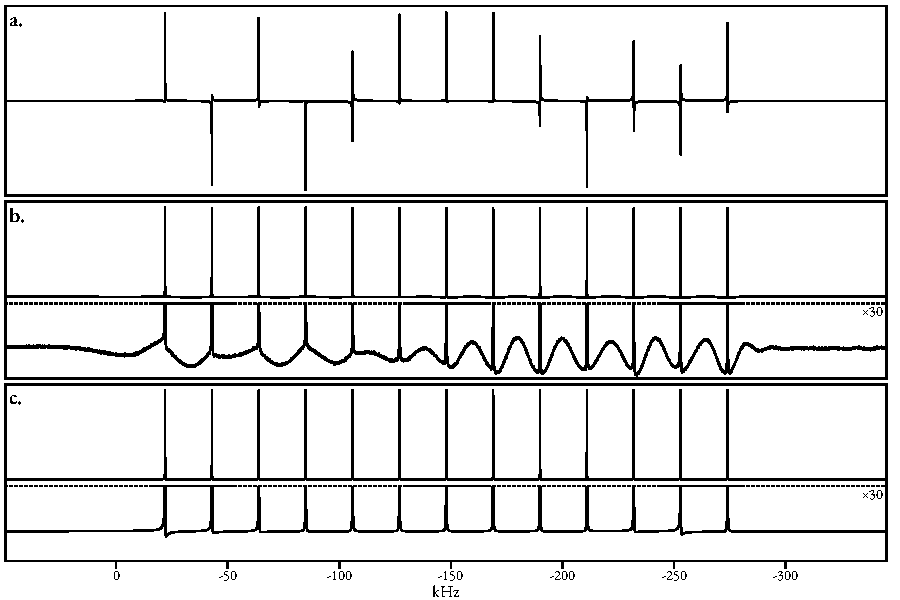
\includegraphics{chirp_phase_vs_estimation_real_data/chirp_phase_vs_estimation_real_data.pdf}
    \caption[
        A comparison of quadratic phase correction vs frequency-dependent
        back-propagation in treating experimental single-chirp excitation data
        generated from a sample of Gd-doped H\textsubscript{2}O in
        D\textsubscript{2}O.
    ]{
        A comparison of quadratic phase correction vs frequency-dependent
        back-propagation in treating experimental single-chirp excitation data
        generated from a sample of 1\% Gd-doped H\textsubscript{2}O in
        D\textsubscript{2}O.
        \textbf{a.} Spectrum generated directly from the acquired \ac{FID}.
        \textbf{b.} Spectrum generated using quadratic phase correction.
        \textbf{c.} Spectrum generated using the back-propagation approach.
    }
    \label{fig:bbqchili-real}
\end{figure}
